\documentclass{article}
\usepackage[utf8]{inputenc}
\usepackage{wrapfig}
\usepackage[parfill]{parskip}

\title{Summary SPMS}
\author{Nicky van Rijsbergen}
\date{October 2014}

\usepackage{natbib}
\usepackage{graphicx}

\begin{document}

\maketitle

\section*{1. Introduction}

\begin{figure}[!h]
\centering
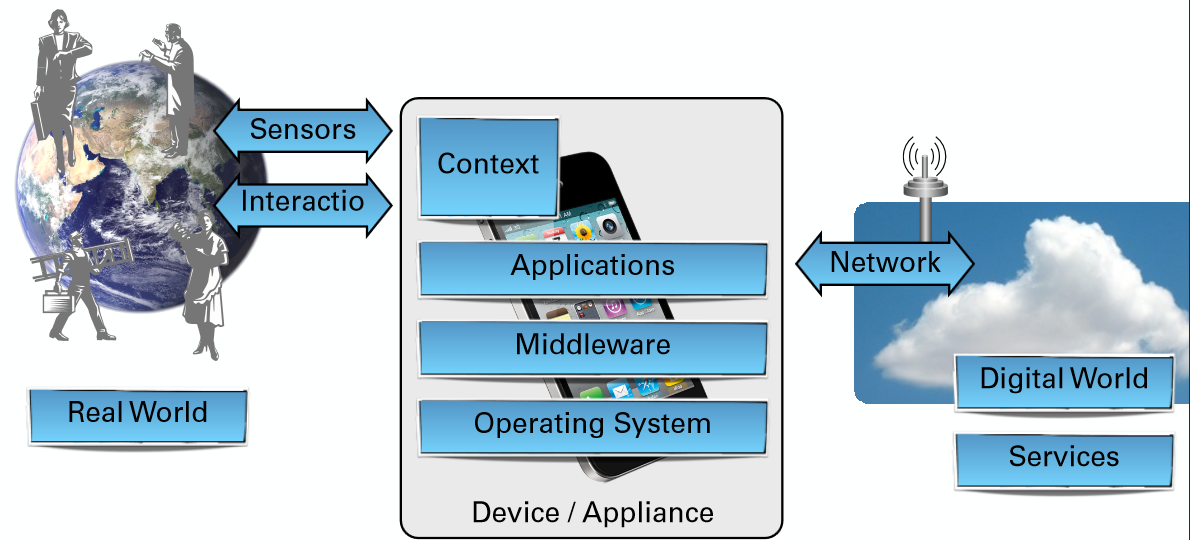
\includegraphics[width=\textwidth, height=\textheight, keepaspectratio]{images/overview_network.png}
\caption{Overview of mobile devices}
\label{fig:overview_mobile_devices}
\end{figure}

Figure~\ref{fig:overview_mobile_devices} gives an overview of mobile devices and communication. Mobile devices have certain resource constraints: battery, CPU, size, HCI and portability are all aspects that need to be taken into account when working with mobile devices. Mobile devices have non-expert users, can be non-interactive, can be used for specialized appliances, can be assistive technology and may contain sensors.

Wireless communication: digital data (1001100) $\rightarrow$ analog signal $\rightarrow$ antenna $\rightarrow$ antenna $\rightarrow$ analog signal $\rightarrow$ digital data (1001100). Between two antennas there can be a lot of obstacles that may block communication, therefor it is challenging to figure out whether communication is possible.

The locking of mobile devices is often susceptible to attacks. These attacks are as simple as just looking at the pattern drawn in the dirt on the screen.

Mobile devices often contain a lot of valuable data. Unfortunately, this data is often not protected well enough. For example account details are stored in the clear. However, this does not really matter as Google (and many other parties) will gather all your information anyway! For tracking your usage they use several identifiers: Device ID/MEI, MAC address, e-mail address, cookies, browser fingerprinting. For tracking your location there are many possibilities: ip-address, GPS, cell-based.

\subsection*{Some attacks on mobile devices}

\subsubsection*{Zeus}
\begin{enumerate}
\item Infect user computer.
\item When user visits banking site, require him to install additional software on mobile device.
\item Zitmo (Zeus in the mobile) sends SMSs to attacker. These may contain mTANs which are required for authentication.
\end{enumerate}
    
\subsubsection*{OV chipcard}
\begin{enumerate}
\item Slice chip layer by layer to reveal internal structure.
\item Reverse engineer the cipher used (crypto-1).
\item Find a flaw in the cipher.
\item Write software to exploit the flaw.
\end{enumerate}
    
\subsubsection*{Passive car key replay attack~\cite{francillon2011relay}}
\begin{enumerate}
\item Trigger car to send a signal.
\item Relay signal to the key.
\item Relay signal from the key to the car.
\item Drive your new car!
\end{enumerate}

\newpage
\section*{4. Bluetooth Security}

\subsubsection*{Some characteristics of bluetooth}
\begin{itemize}
\item 2.4GHz ISM band, class 1 up to 100m, class 2 up to 10m and class 3 up to 1m. (range can be extended with high-gain antennas and amplifiers, so the range should not be considered as secure)
\item Security goals: confidentiality, authentication, authorization.
\item Threats: eavesdropping, man in the middle attacks, denial of service.
\end{itemize}

Bluetooth comes with built-in security. There are several modes which will be described below. In the end only mode 4 can be secure and all other modes can easily be broken.

\begin{itemize}
\item Mode 1 (BT $<$ 2.0): No security.
\item Mode 2 (BT $<$ 2.0): Service-link security, enforced after link establishment, can be configured per service.
\item Mode 3 (BT $<$ 2.0): Link-layer security, PIN authentication, encryption, enforced during link establishment.
\item Mode 4 (BT $>$ 2.1): Secure Simple Pairing, service-level security.
\item Cryptographic primitive: modified SAFER+ uses 128 bit key and 128 bit blocks.
\end{itemize}

\begin{wrapfigure}[8]{l}{5.5cm}
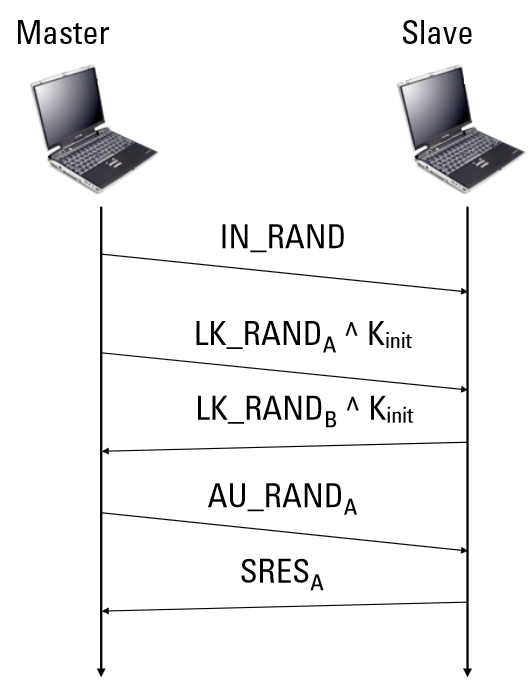
\includegraphics[width=5.5cm]{images/bt_communication_20.png}
\caption{Initial communication to set up bluetooth communication}
\label{fig:bt_communication_2.0}
\end{wrapfigure} 

\hspace{0.5cm}
\subsubsection*{Steps}
If $K_{AB}$ is known, then skip to step 3
\begin{enumerate}
\item $K_{init}$ is generated from $IN\_RAND$, $PIN$ and $MAC_{master}$.
\item Link key $K_{AB}$ is generated from $LK\_RAND_{A}$, $LK\_RAND_{B}$, $K_{init}$ and MACs.
\item Challenge response authentication: slave authenticates to master with $AU\_RAND_A$, $K_{AB}$ and $MAC_B$.
\end{enumerate}




\newpage

The only secret in this entire communication is the PIN code used. This PIN can easily be bruteforced~\cite{shaked2005cracking}:

\begin{enumerate}
\item Guess a PIN, i.e. 0000.
\item Calculate hypothesis for $K_{init}$ and $LK\_RANDs$.
\item Use $LK\_RAND$ values to calculate $K_{AB}$.
\item Use $AU\_RAND$ values to calculate $SRES_A$ from $K_{AB}$.
\item $SRES_A$ incorrect? Step 1. Correct? You win life.
\end{enumerate}

This can however only be done during the initialisation phase. Luckily there are three ways to retrigger an initialisation phase. 

\begin{itemize}
\item Inject $IN\_RAND$ which makes the slave think that the master has lost the key.
\item Spoof several invalid $SRES_A$ values after which the master will revert to pairing.
\item Spoof $LMP\_not\_accepted$ message.
\end{itemize}

Besides this bruteforce attack on the PIN, there are many more attacks possible on BT $<$ 2.0. Obviously we need a new protocol to initialise communication. We will now get into BT 2.1. This version makes use of Elliptic Curve Diffie Hellman to exchange keys. Several pairing models have been proposed to improve security of the protocol:

\begin{description}
\item[Numeric Comparison] display 6-number value that users need to compare. Knowing this value does not reveal key. See figure~\ref{fig:bt_authentication_2.1} for an example protocol. 
\item[Passkey Entry] First device displays a value that needs to be entered in the second device. Knowing value does not reveal key.
\item[Just works] is like numeric comparison but without displaying the value. No MitM protection though.
\item[Out Of Band] means that a different channel which is assumed secure is used for communication. For example NFC.
\end{description}

\begin{figure}[!h]
\centering
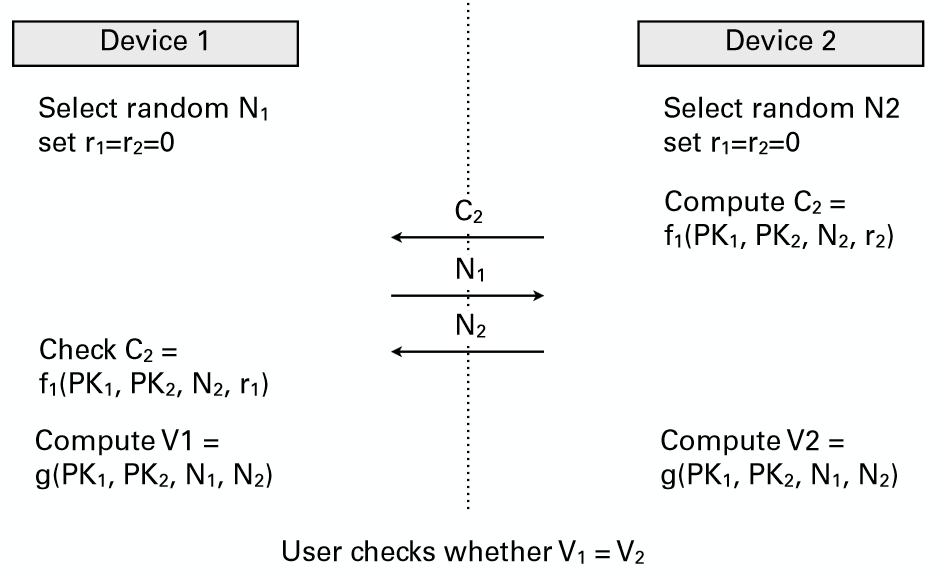
\includegraphics[width=\textwidth, height=\textheight, keepaspectratio]{images/bt_communication_21.png}
\caption{Example authentication BT 2.1: numeric comparison}
\label{fig:bt_authentication_2.1}
\end{figure}

Another version of Bluetooth has been developed, called BT 3.0 high speed. This version is basically always high on speed and cocaine. Thanks to all these drugs this version is able to make use of an alternate MAC/PHY. It can for example make use of a present 801.11 network. The bluetooth link is used for authentication, again the same pairing mechanisms can be used. After authentication, the alternate medium is used for the actual communication

An inevitable consequence of the abusive use of drugs is low energy. To counter this problem another version of Bluetooth had to be developed, namely BT 4.0 low energy. This version can use the same pairing models as BT 2.1 except for numeric comparison. It also has NO Diffie-Hellman key agreement as it still owes Diffie a lot of drug money and we all know what Diffie does to people that do not pay!

\begin{figure}[!h]
\centering
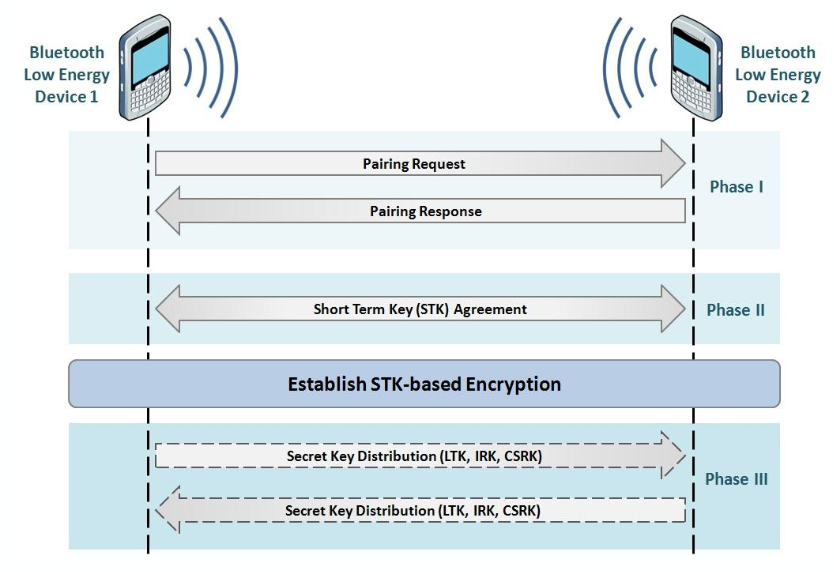
\includegraphics[width=\textwidth, height=\textheight, keepaspectratio]{images/bt_communication_40.png}
\caption{Communication BT 4.0 LE}
\label{fig:bt_authentication_4.0}
\end{figure}

At first a temporary key is sent. With Passkey Entry this is a value between 0 and 999999, with Just Works this is 0 and with OOB this is a 128 bit value. Then each device confirms $E_{TK}(Rand, PairingMessages, Addresses)$ and they reveal Rand if this can be confirmed. Then a Short Term Key is calculated: STK = $E_{TK}(S_{Rand} || M_{Rand})$. Only OOB will probably provide some security (confidentiality and authentication) as the other two provide a TK that is easily guessable. Figure~\ref{fig:bt_authentication_4.0} gives an overview of 

\section*{5. Security of GSM/UMTS/LTE}
The network of GSM consists of several parts. I think that figure \ref{fig:gsm_network_architecture} gives a nice overview and below is short description of every part.

\begin{itemize}
\item ME (Mobile Device) identified by IMEI
\item SIM is identified by IMSI.
\item ME and SIM communicate with BTS (Base Transceiver Station). The BTS is responsible for one cell and within this cell all ME will communicate with this BTS.
\item BTS (Base Station Controller) controls the BTS. The BSC and BTS combined are called the BSS (Base Station Subsystem).
\item The MSC (Message Switching Center) takes care of routing to other networks and controls the connections.
\item The VLR (Visitor Location Register) has information about the participants of the connections and takes care of authentication.
\item The HLR (Home Location Register) is like the VLR but stores all the subscriber data permanently.
\item The EIR (Equipment Idendity Register) stores all EMEI which can be used to trace stolen devices.
\item The AuC (Authentication Center) takes care of authentication parameters and encryption.
\end{itemize}


\begin{figure}[!h]
\centering
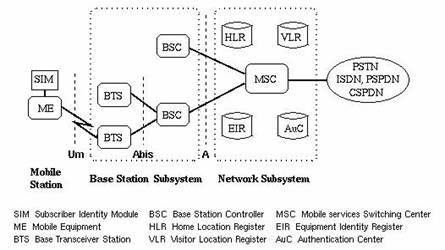
\includegraphics[width=\textwidth, height=\textheight, keepaspectratio]{images/GSM_Network_Architecture.jpg}
\caption{Overview of GSM network architecture}
\label{fig:gsm_network_architecture}
\end{figure}

\subsection*{GSM Security}
A3 is used for authentication and a combination of A5 and A8 are used for encryption. Figure~\ref{fig:gsm_auth_enc} gives a nice overview of the authentication and encryption protocols. 

\begin{figure}[!h]
\centering
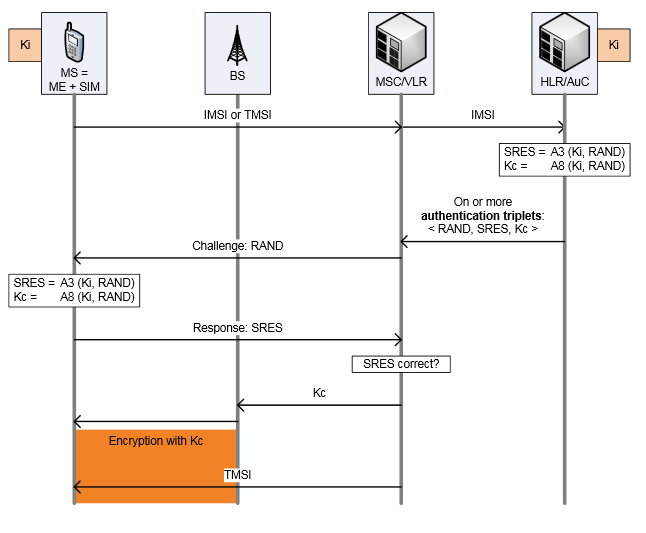
\includegraphics[width=\textwidth, height=\textheight, keepaspectratio]{images/gsm_auth_enc.png}
\caption{GSM Authentication and Encryption protocols}
\label{fig:gsm_auth_enc}
\end{figure}

There are however quite a few security issues with GSM.

\begin{itemize}
\item The IMSI is sent in the clear and can be caught. Also the base station is never authenticated. I think this implies that an attacker can pretend to be in any cell he wants to be. It also allows an attacker to track a user.
\item COMP128 used in SIM has flaws which allows an attacker to retrieve the unique key stored on the SIM. Once the key has been retrieved an attacker can clone the SIM. You need to try about 150.000 challenges to successfully brute force the unique key.
\item A5-x has some flaws. A5-0 has no security. A5-1 is the first normal version used in many countries. A5-2 is the deliberately weakened version. A5-3 is modified such that it can use the Kasumi cipher. These modifications have however weakened this version, which makes it unsafe to use. A5-4 uses an 128 bit key. A5-2 can be attacked with chosen plain texts. As of 2009 A5-1 should not be used either as rainbow tables have been developed for easy cracking.
\item P2P links in the backend are often not encrypted, which allows the eavesdropping of $K_c$, Rand and SRES.
\end{itemize}

\subsection*{3G Security}
Some security enhancements of 3G are: 

\begin{itemize}
\item Mutual authentication via authentication and key agreement. Use of message sequence number to prevent replay attacks.
\item Stronger confidentiality and integrity by specific data algorithms with stronger keys.
\item Protection of communication in the core network.
\item Users can see and configure security settings.
\end{itemize}

Below you see the 3g protocol. In order to prevent tracking based on IMSI the VLR sends an IMSI request. The attacker can however spoof a request and thereby still track a user. 

\begin{figure}[!h]
\centering
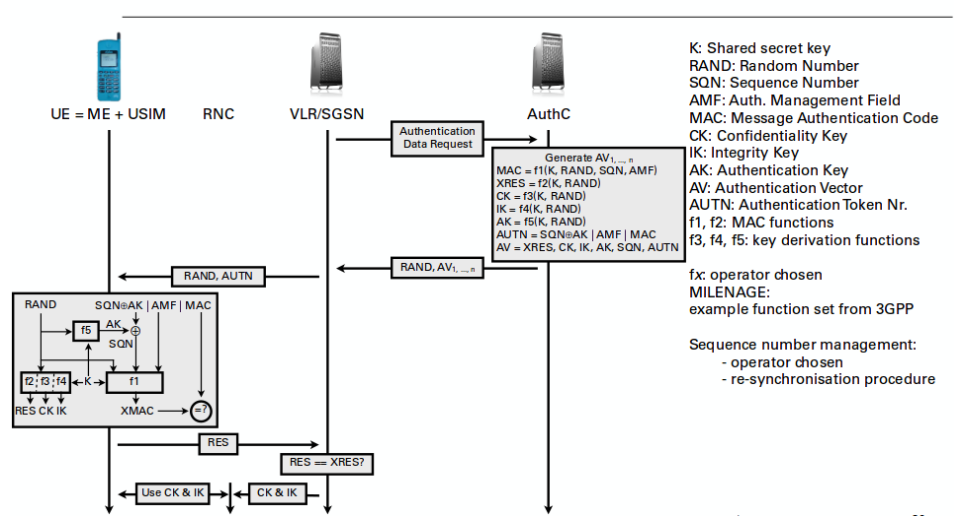
\includegraphics[width=\textwidth, height=\textheight, keepaspectratio]{images/3gprotocol.png}
\caption{Protocol 3g}
\label{fig:3gprotocol}
\end{figure}

LTE security is similar to 3G but there are some differences. First of all the keys used can be up to 256 bits instead of 128 bits. Secondly there is an extended key hierarchy for fast hand-overs. Thirdly it requires the use USIM instead of SIM. There are some other differences which I do not consider important.

Some weaknesses that still exist in 3G/LTE.

\begin{itemize}
\item IMSI is still sent in the clear.
\item IMEI still not authenticated.
\item Non-repudation for costs is still based on server logs. No public-key signatures.
\item DoS attack: spoof of de-registration request and spoof of other location.
\end{itemize}

\subsubsection*{Brute force trade-off}
When attacking a cipher there is a trade-off between runtime and storage usage. A way to reduce storage usage is to use hash chains. A problem with hash chains may have collisions which will lead to the same chain, but take twice the storage. Distinguished Codepoints is a technique that skips computing intermediate values if you have already computed the final value. Rainbow tables can be used to prevent the collision of chains, because it uses different reduction functions every step. Example:

\begin{description}
\item[Hash chain] Plaintext $R_0 \rightarrow$ Hash1 $R_0 \rightarrow$ Hash2 $R_0 \rightarrow$ Final Hash
\item[with Rainbow tables] Plaintext $R_0 \rightarrow$ Hash1 $R_1 \rightarrow$ Hash2 $R_2 \rightarrow$ Final Hash
\end{description}

\section*{6. Security of RFID/NFC}
RFID stands for radio frequency identification which can be used to read and store data contactless. Some applications of RFID: tagging and tracking of goods and money, access control, electronic passports, localisation, anti-spoofing. An RFID consists of a battery, an antenna, a substrate and a chip. The energy supply can be

\begin{itemize}
\item Passive: reader signal is used for chip operations and transmission.
\item Semi-active: battery is used for chip operations and reader signal is used for transmission.
\item Active: battery is used for chip operations and transmission.
\end{itemize}

\subsection*{NFC}
NFC is a set of standards for communication between cellphones, readers and passive tags. Practical distance is 4-10cm and it operates at 13.56 MHz with possible data rates of 106, 212 and 424 Kbit/s. Some applications are ticketing, payment, access control.

\begin{itemize}
\item Passive communication: initiator creates a field and the target modifies this field to respond.
\item Active communication: both parties create their on field alternately.
\item Active-Active: two NFC devices talk.
\item Active-Passive: NFC device reads RFID tag.
\item Passive-Passive: NFC device acts as RFID tag.
\end{itemize}

\noindent There are some threats to NFC:

\begin{itemize}
\item Eavesdropping: 15 meter with active mode and 1.5 meter with passive mode.
\item Jamming
\item Modification by flipping some bits
\item Man in the Middle although this is very hard in practice due to collision detection.
\item NFC specific key agreement may leak key with random noise.
\end{itemize}

\noindent Because of these threats there are several attacks possible, namely relay, replay, and side-channel attacks. Additionally one can attack the crypto used and one can trace the user.

Some problems with NFC are that the standard proposes no authentication and encryption schemes. Also privacy may be an issue as these tags may reveal the ID.

Figure \ref{fig:crypto1overview} gives an overview of the crypto-1 cipher which was used in MIFARE classic. The LFSR has a weak random number generator. Another weakness is the 16 bit random number and the authentication protocol leaks keystream.

\begin{figure}[!h]
\centering
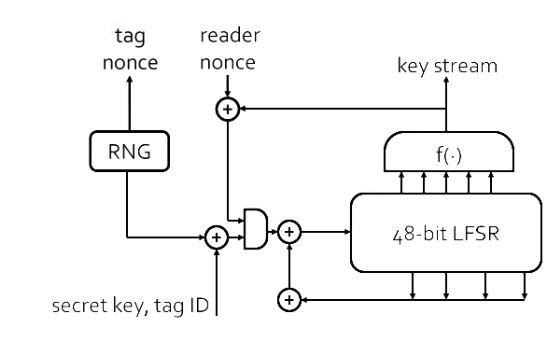
\includegraphics[width=\textwidth, height=\textheight, keepaspectratio]{images/crypto1overview.png}
\caption{Crypto-1 overview}
\label{fig:crypto1overview}
\end{figure}

\section*{7. Wireless Sensor Networks}
A wireless sensor network is a collection of autonomous sensors that measure conditions such as temperature, sound and pressure and send this data to a main location where the data will be evaluated. Modern WSNs are also capable of controlling the sensors. WSNs have quite a few security requirements:

\begin{itemize}
\item Availability, Authentication, Authorization, Confidentiality, Integrity, Non-repudiation, Freshness.
\item Forward secrecy: cannot read future messages after leaving the network.
\item Backward secrecy: cannot read past messages after joining the network.
\end{itemize}

Some security challenges that need to be overcome are key distribution, secure routing, secure data aggregation, secure and reliable clustering and trust management. 

\subsection*{Attacks on WSN~\cite{wang2006survey}}

\begin{itemize}
\item Jamming of nodes. Can be prevented by spreading the spectrum of communication.
\item Tampering attack: attacker gets access to a node. Can be prevented by detecting tampering and reacting properly to it.
\item Exhaustion by overloading a node and thereby emptying battery. Prevent this by rate limitation.
\item Collision attack, try to interfere with packet transmissions.
\item There are also some attacks possible on routing. A malicious node may drop all or some communication. It could also rush communication to get malicious packets through faster. Some other routing attacks are when an attacker pretends to have many identities or when an attacker creates a fast out of band connection which lures are communication to that node (wormhole-attack).
\end{itemize}

As key management can be quite hard with many different sensors all around the field, Eschenauer and Gligor have come up with a way to solve this. There are basically $N$ different keys in the key pool. Every node will get $m$ keys assigned. Then if two nodes have a matching key they can connect to each other. Also if node A and node B share a key and node B and node C share a key, then node A and node C can talk. Figure \ref{fig:egkeydistribution} gives an overview. 

\begin{figure}[!h]
\centering
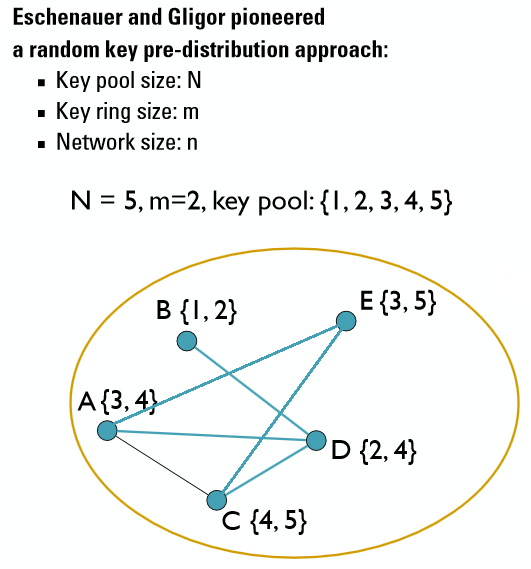
\includegraphics[width=\textwidth, height=\textheight, keepaspectratio]{images/eg_keydistribution.png}
\caption{Eschenauer and Gligor key distribution}
\label{fig:egkeydistribution}
\end{figure}

A problem with this system is that once a node has been compromised, then all the nodes that it shares a key with, will also be compromised. q-composite scheme tries to restrain this danger by enforcing that two nodes share at least $q$ keys. Multi-path key reinforcement tries to counter this attack by computing another key between every two nodes.

Concluding we can say that the EG key distribution scheme is scalable (10 to 100.000 nodes), flexible (saves money and can be used in many different environments) and secure (compromise of keys effect few links and revocation and rekeying is easy).

Another way to distribute keys among many sensors is the uTesla broadcast authentication. Use a one way function $F$ to compute $F(K)$, $F(F(K))$, $F(F(F(K)))$, etc. The base station has K and every next station will have $F^{n}(K)$ where n depends on the position in the chain. A disadvantage of this method is that it may take a while to distribute the keys.

\newpage
\section*{8. Vanet Security}
A vehicular ad hoc network (VANET) is a network in which each car is turned to a wireless router. Cars can join and leave the network, connecting all cars in the network with each other. There are three applications of vehicular communication: safety, efficiency and comfort. An example of safety may be that cars can communicate where an accident has taken place. For Vanets we can use different communication patterns to establish the network~\cite{schoch2008communication}.

\begin{description}
\item[Beaconing] is a technique where every car is periodically updating all neighbouring nodes of it's current status. This technique is mostly used to send some basic information that has no real priority.
\item[Geobroadcasting] is immediate distribution of information in a large area, for example, to inform approaching vehicles of a sudden event.
\item[Unicast Routing] is sending a message through the ad hoc network to reach a specific target. These messages will mostly be about internal system events or manually triggered events. This technique will probably not be used for security.
\item[Advanced Information Dissemination] is spreading the message to all the relevant nodes based on the context. The messages will be queued up and communication is one directional.
\item[Information Aggregation] is much like dissemination, but now information is processed. This allows cars to compress messages if necessary, which in turn allows a more effective use of the bandwidth. In contrast to dissemination, messages are first processed and then sent again.
\end{description}

There are many threats to Vanets:

\begin{description}
\item[Availability] Denial of Service.
\item[Integrity] Masquarade, manipulation, replay, insertion of information.
\item[Authenticity] Manipulation, masquarade.
\item[Confidentiality] Eavesdropping, traffic analysis.
\item[Non-repudiation] Repudiation
\end{description}

In order to achieve security in vehicular communication, the following approach is suggested: first achieve id management and message integrity, secondly protect privacy and finally detect misbehavior.

With Vanet there is a scalability problem, when many cars get together (i.e. a traffic jam) then all these cars have to verify every message that is being sent. To counter this we need an efficient crypto that creates small signatures. Additionally we can design a chip that can cope with all the computations or we can reduce the security requirements. We can for example selectively send the certificate instead of adding it to every message. Some possibilities:

\begin{description}
\item[Periodic omission of certificates] is to add a certificate every n beacons. It can occur that a vehicle has to wait for n - 1 beacons to get a certificate. All communication before the certificate has been received, will be dropped.
\item[Neighbor-based Certificate omission] is to add a certificate if the list of neighbours changes. So when a new vehicle enters the network, you send the certificate. The problem with this approach is that it does not scale well.
\item[Congestion-based certificate omission scheme] is basically about omitting certificates when it is necessary, for example when you notice a congestion.
\end{description}

\subsection*{Privacy}

Although privacy is a joke, we may still consider building in privacy in V2V communication. A way to counter this, is to use pseudonyms. Every car will get a pseudonym for a certain period, after which it will get a different pseudonym. This will create privacy, but this also means that law enforcement does not know who's car it is. A way to solve this problem is to store the car\_id and pseudonyms combination at the pseudonym provider. The C2C-CC has proposed a PKI structure, which is summarized by figure~\ref{fig:c2cccpki}.

\begin{figure}[!h]
\centering
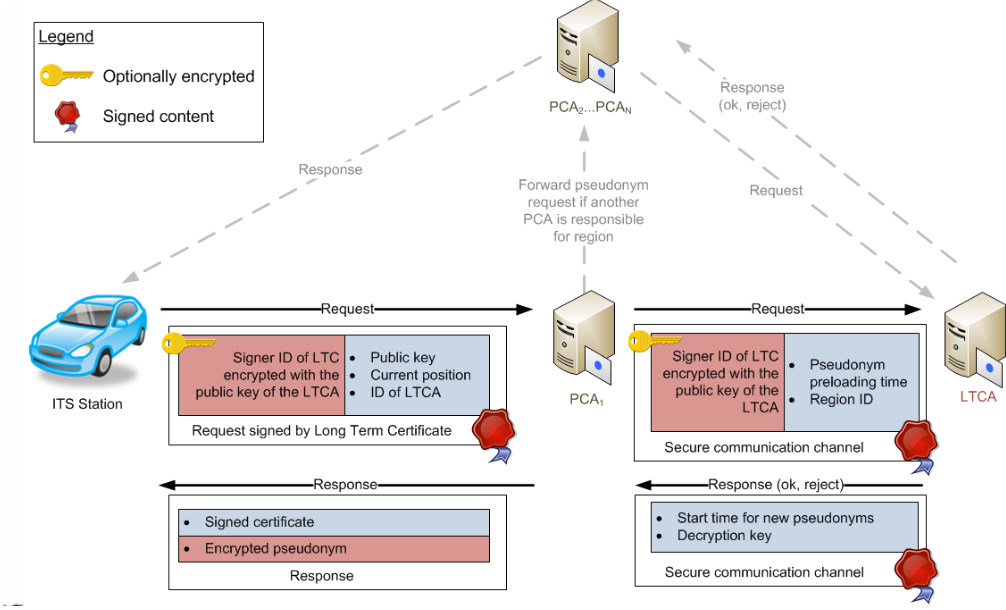
\includegraphics[width=\textwidth, height=\textheight, keepaspectratio]{images/c2cccpki.png}
\caption{C2C-CC - PKI}
\label{fig:c2cccpki}
\end{figure}

A system that makes use of tokens has been proposed to issue pseudonyms. First the car acquires tokens from the CA using the blind signature scheme. Secondly the car can spend a token to acquire pseudonym certificates. Finally these pseudonyms can be used to authenticate messages to other cars.

\bibliographystyle{plain}
\bibliography{references}
\end{document}
